% \begin{figure}[htp] \centering
%     \begin{subfig}[width=0.40\columnwidth]{width=0.40\columnwidth}
%         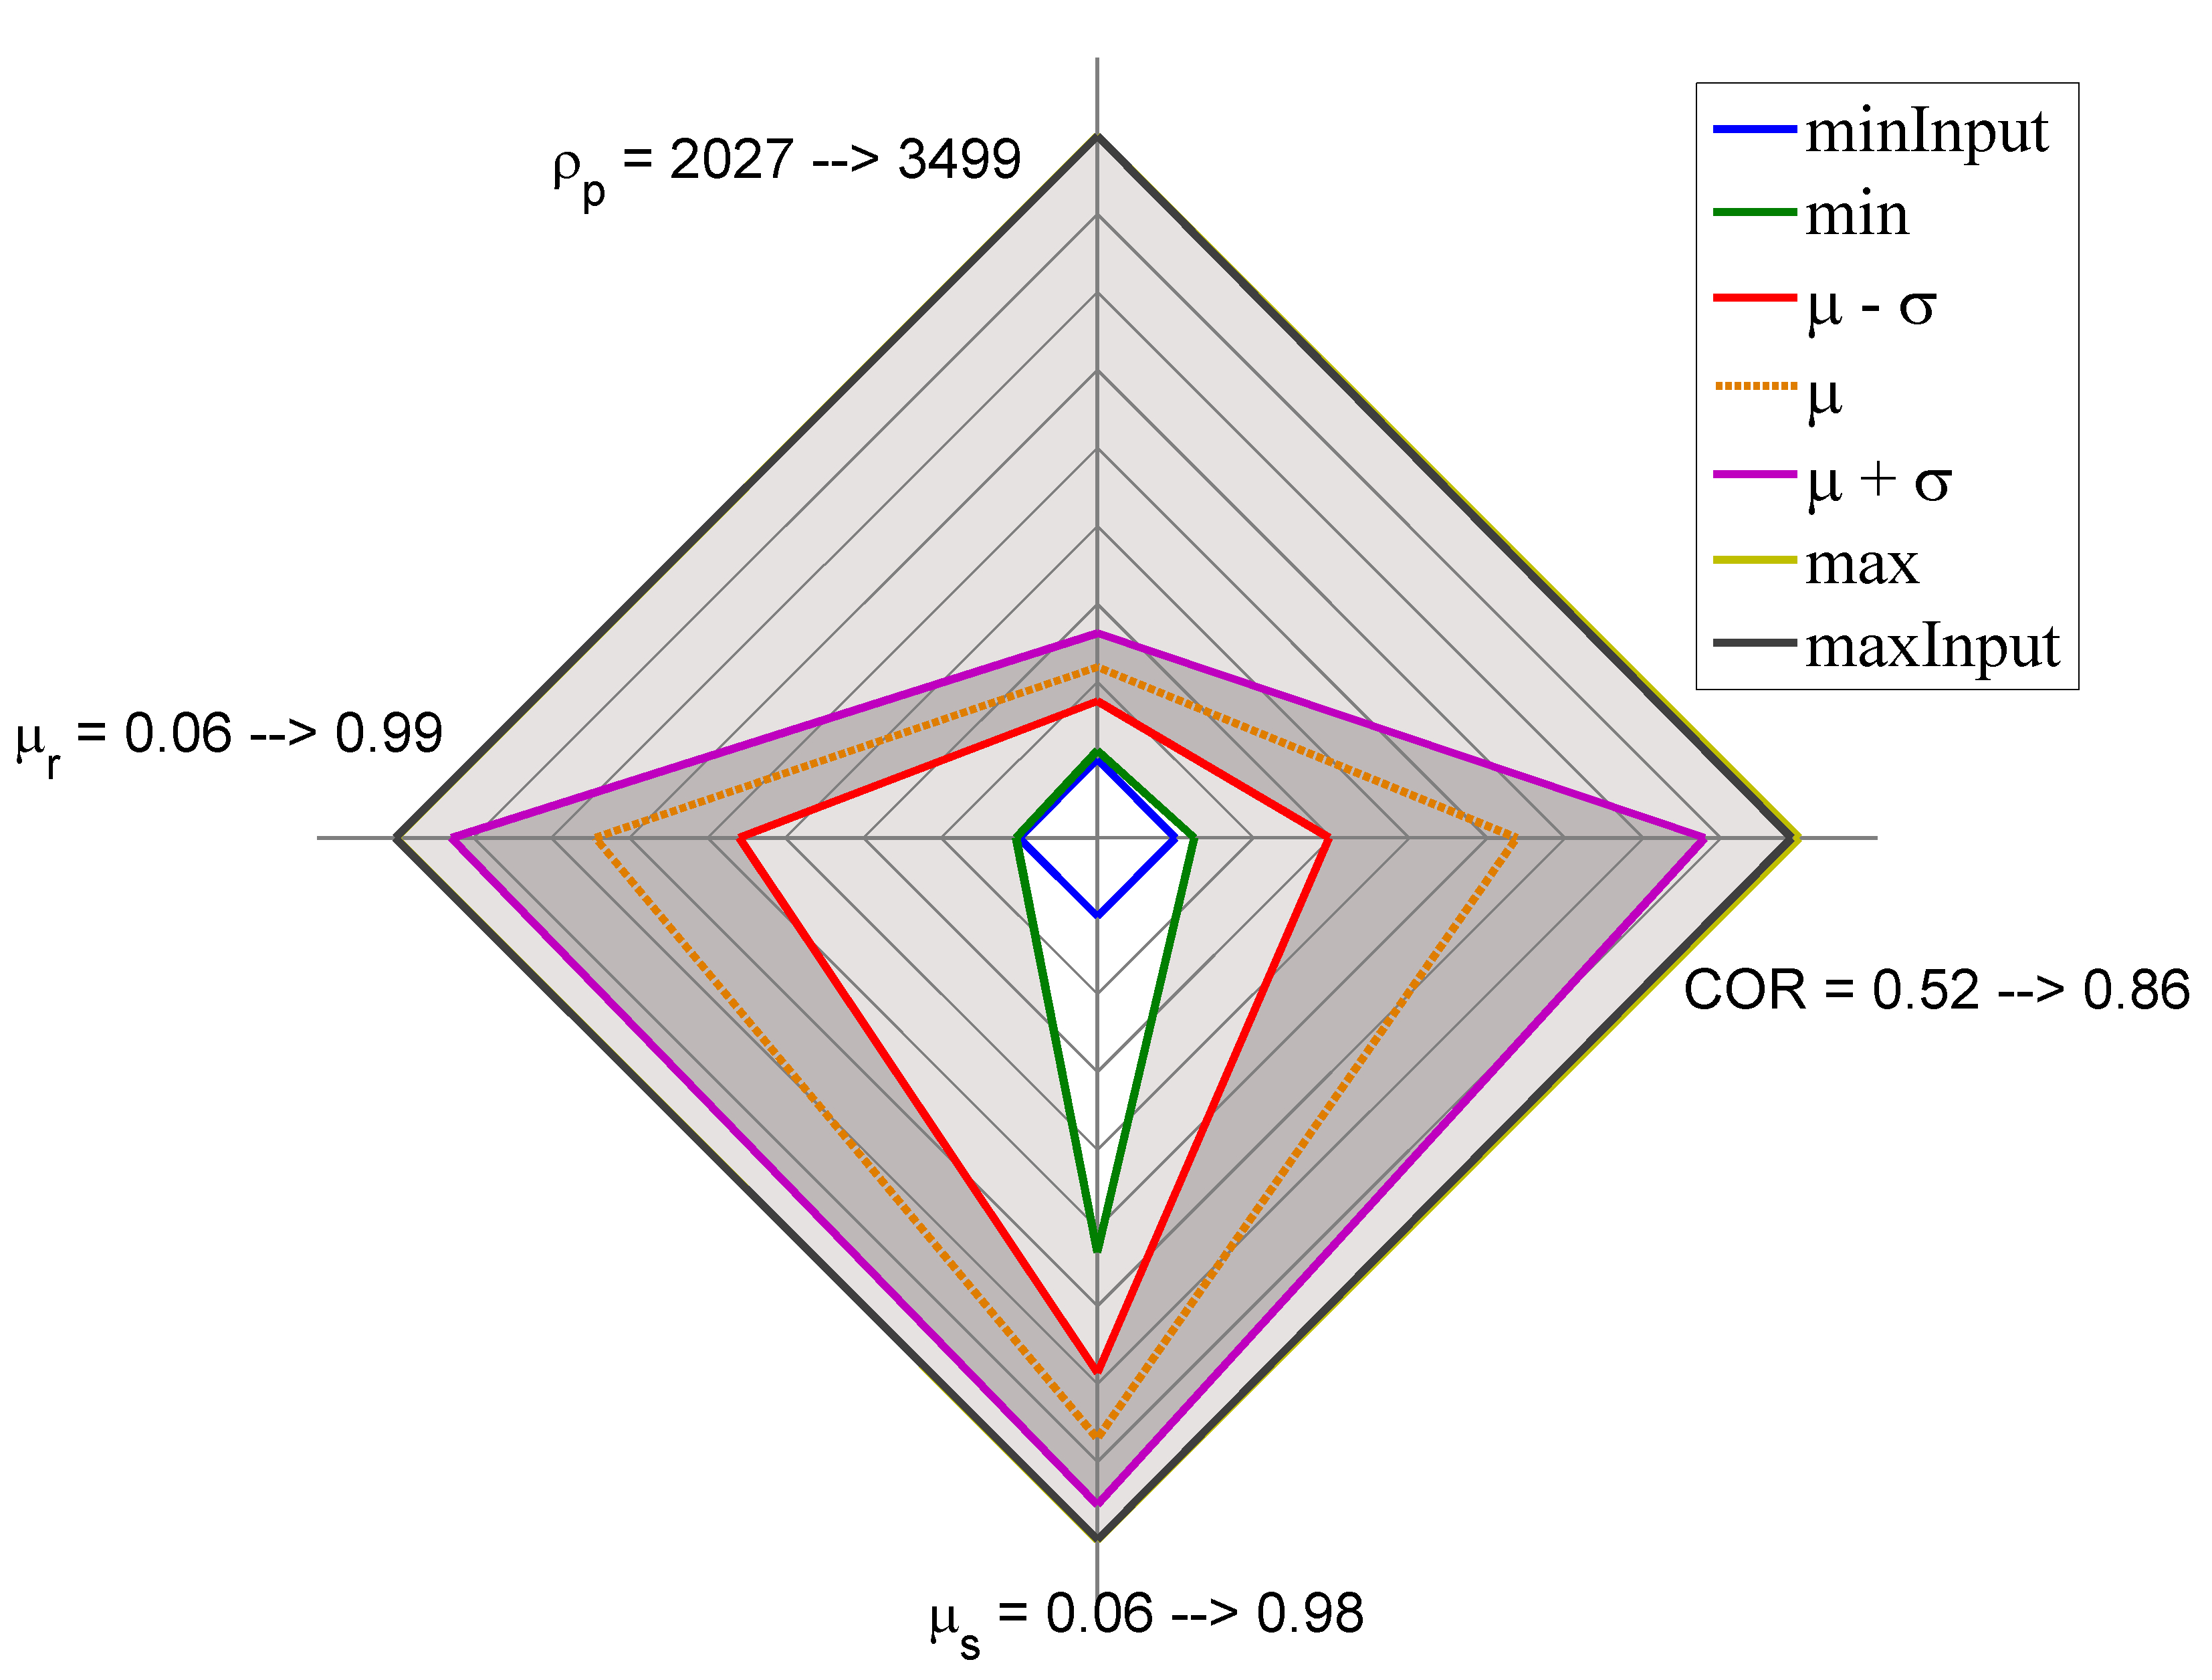
\includegraphics[width=\textwidth]{images/original/24radarpirker1schulze10070}
%         \caption{Cloud plot, $AOR_{exp} = 38.85 ^\circ$}
%         \label{fig:32cloudpirker1aor} 
%     \end{subfig}\ \quad
%     \begin{subfig}[width=0.40\columnwidth]{width=0.40\columnwidth}
%         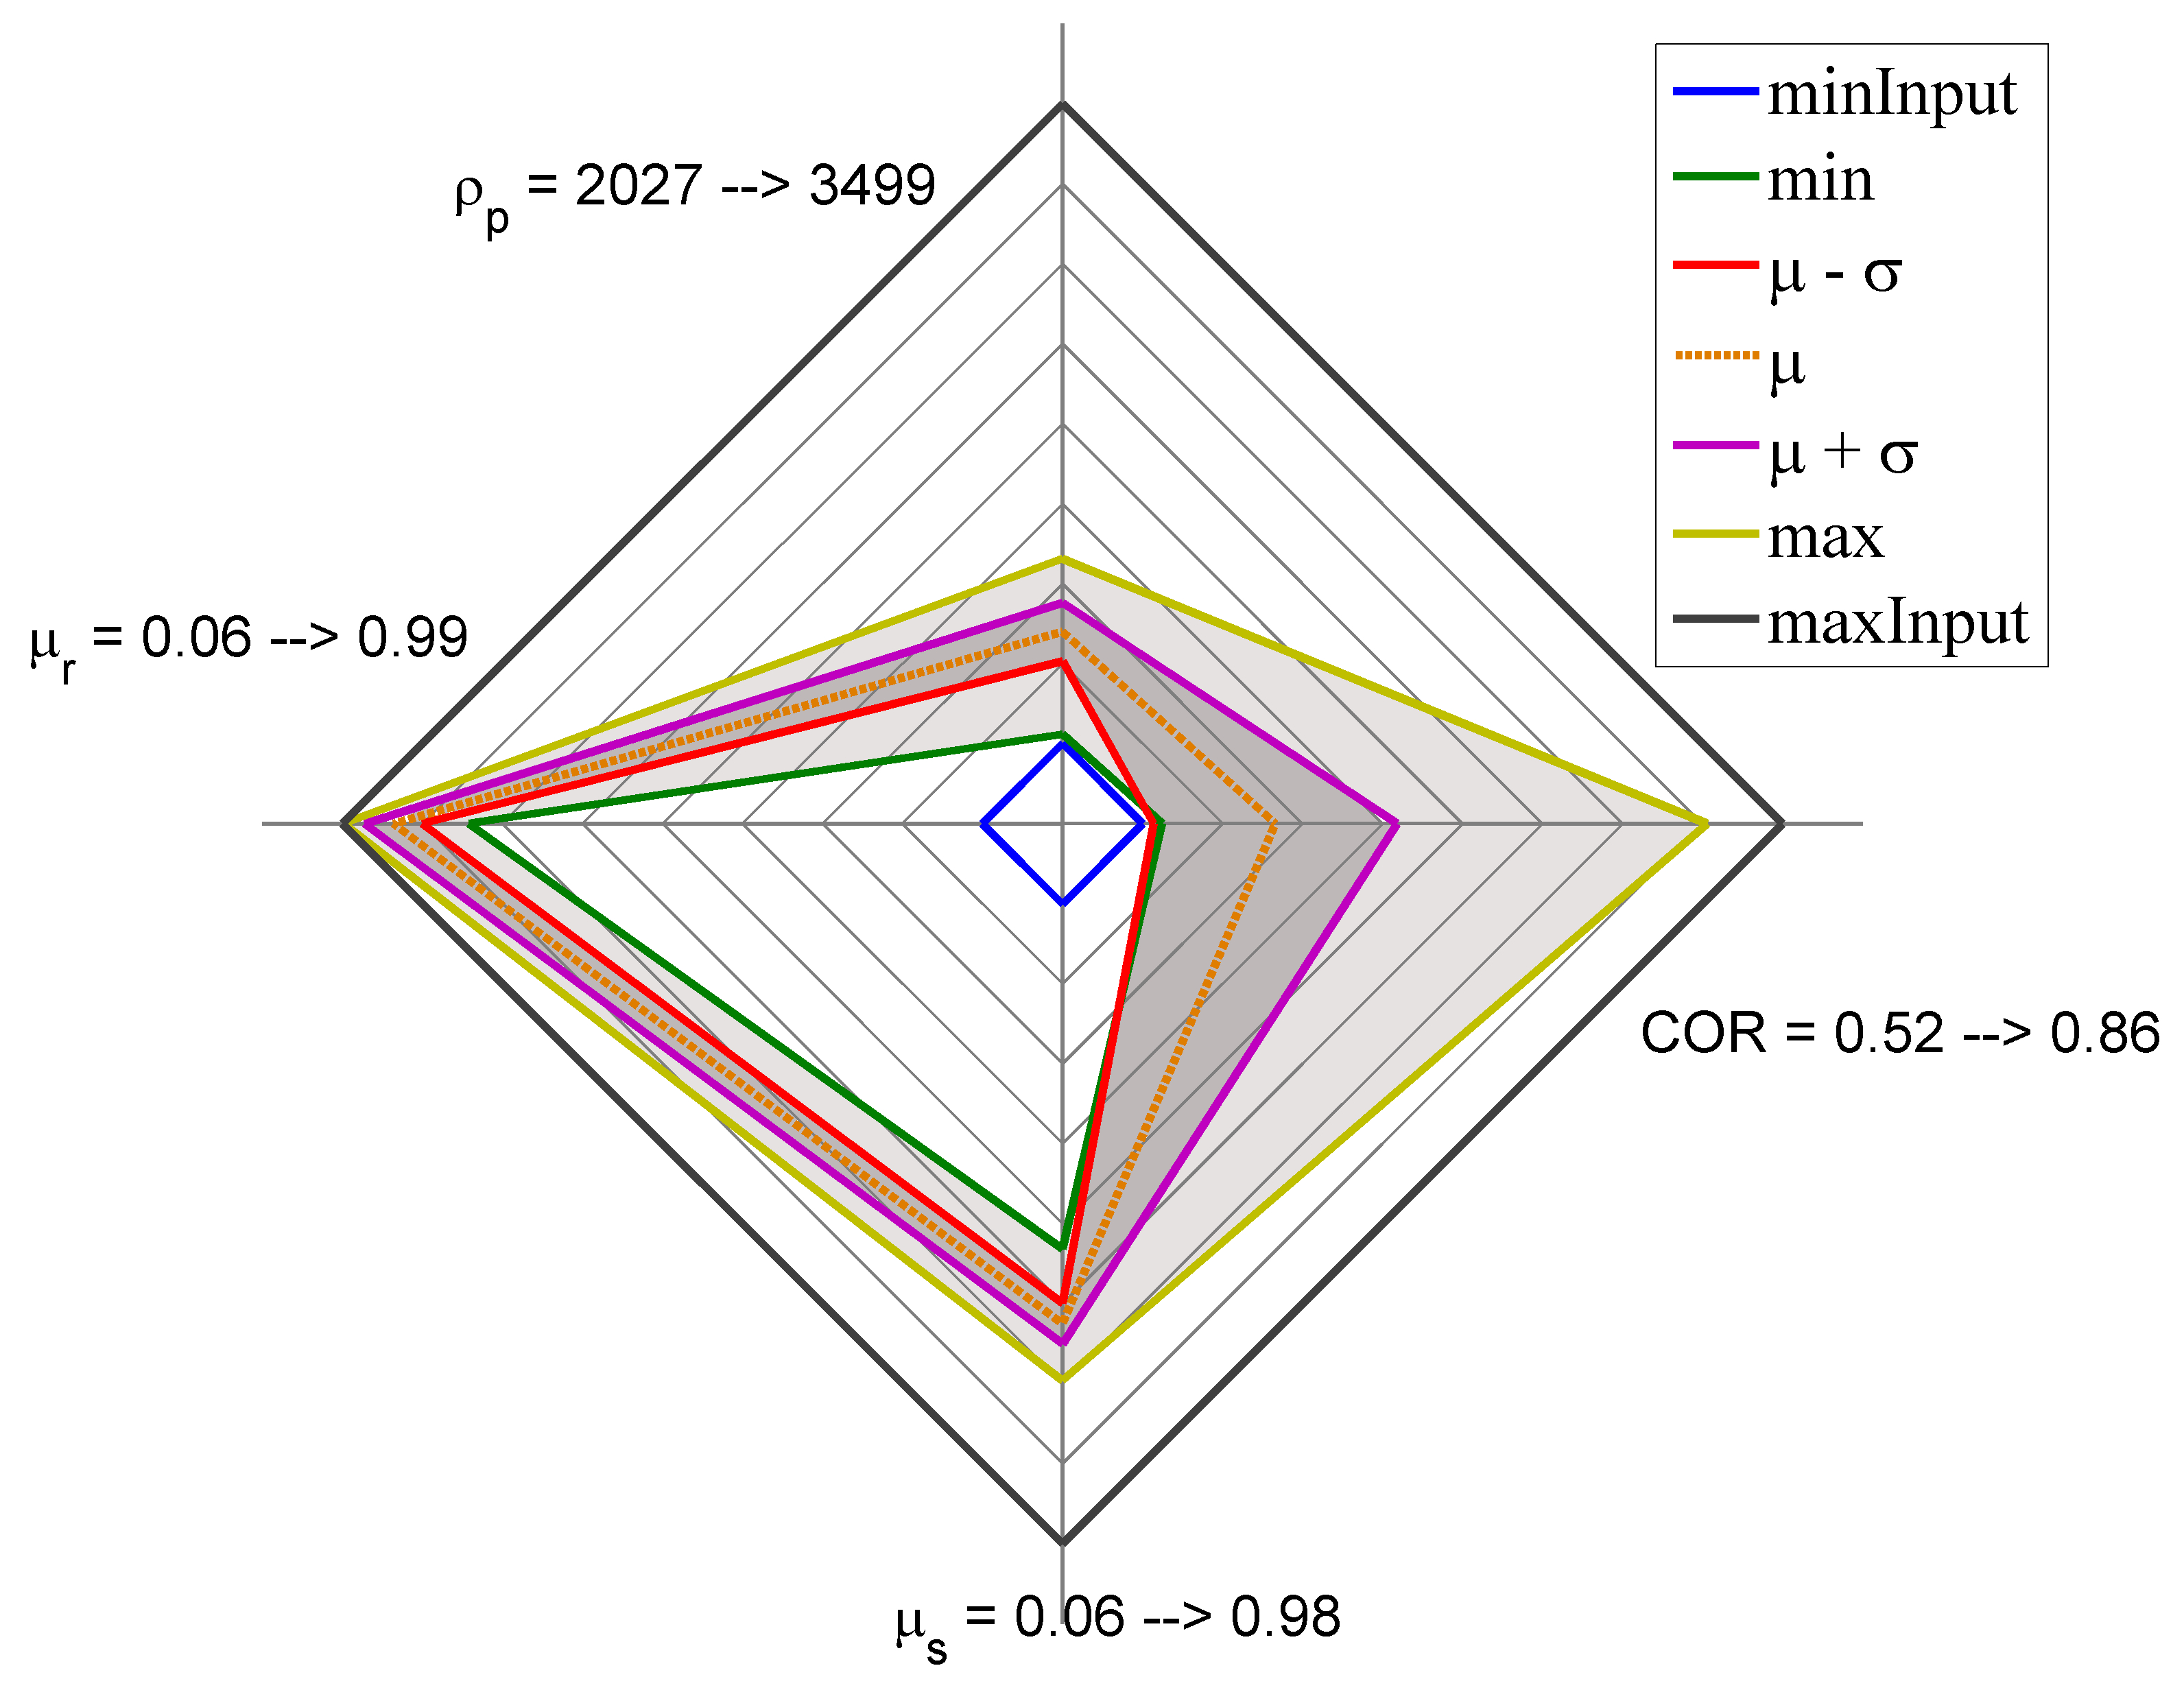
\includegraphics[width=\textwidth]{images/original/33radarpirker1schulze10070aor}
%         \caption{Cloud plot, $AOR_{exp} = 38.85
%         ^\circ$ \& $SCT$: $\sigma_n=10070 ~[Pa]$}
%         \label{fig:34cloudpirker1schulze10070aor} 
%     \end{subfig}
%     \caption{Density plot comparison of AOR and SCT results}
%     \label{fig:35schulze10070aorradarandcloud}
% \end{figure}

\begin{figure}[tb]
\centering
\subfloat[Radar Schulze 10070 Pa]
{\label{fig:24radarpirker1schulze10070}%
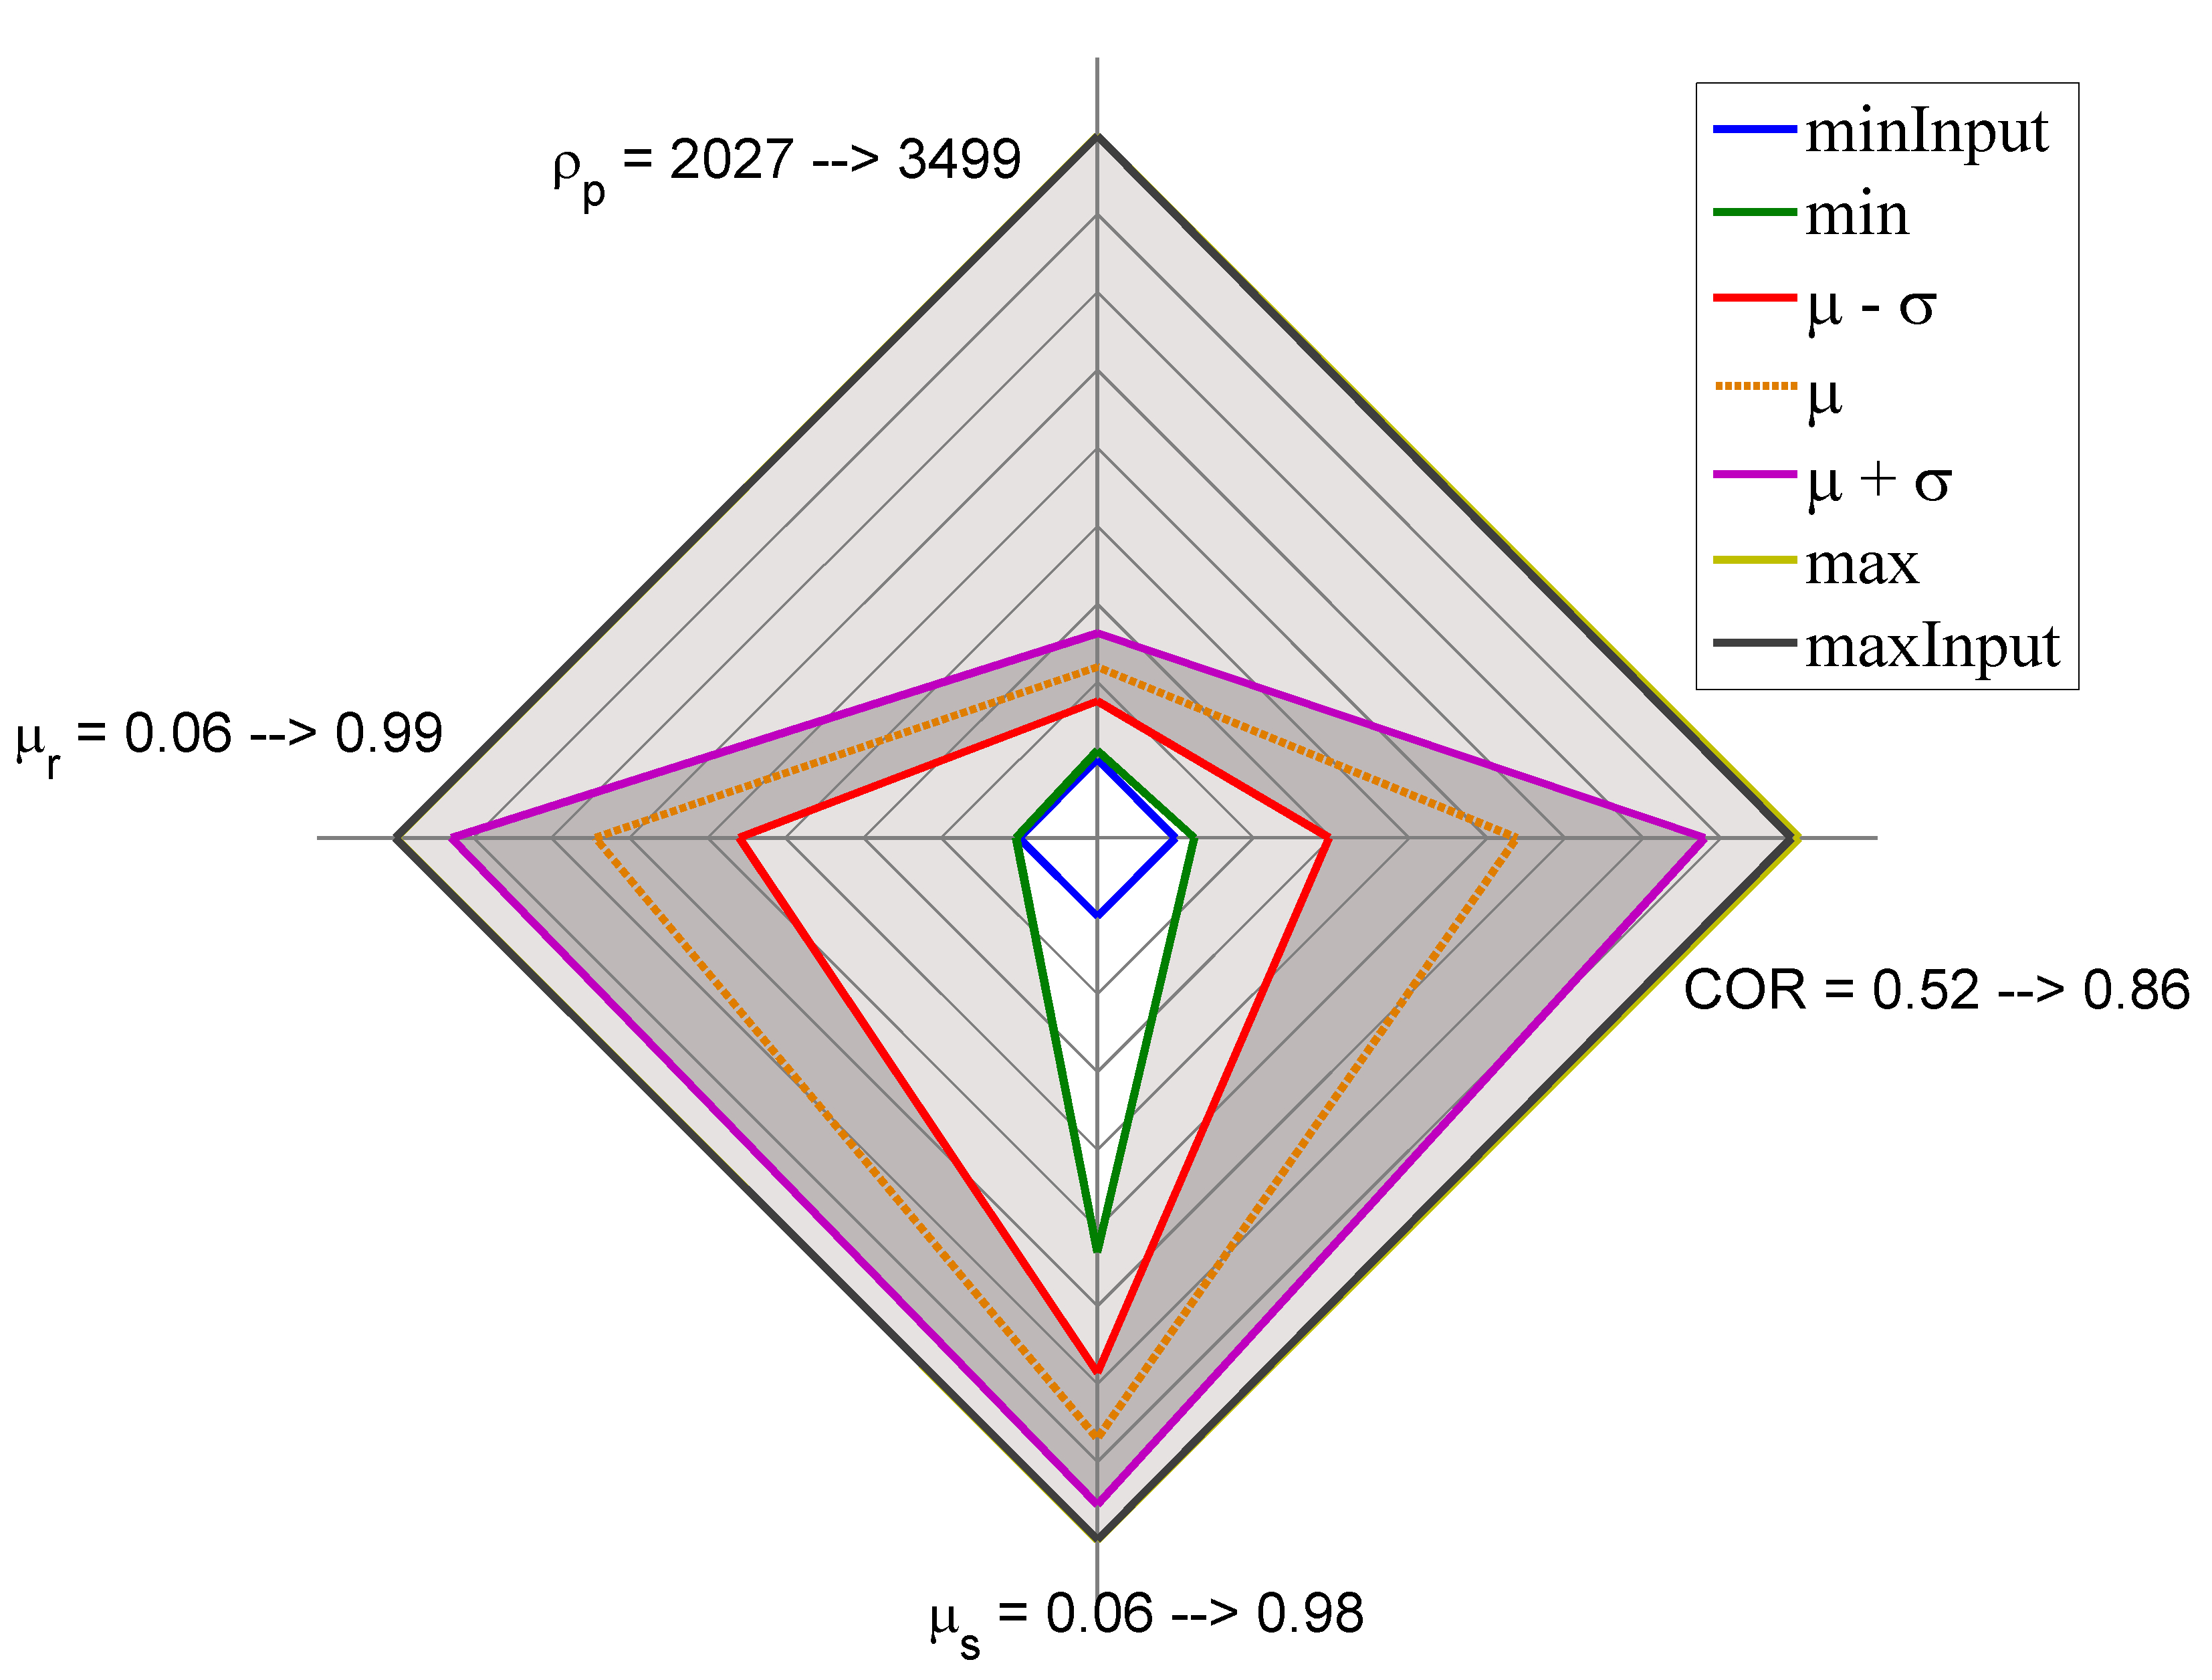
\includegraphics[width=.45\columnwidth]{images/original/24radarpirker1schulze10070}} \quad
\subfloat[Radar Schulze 10070 Pa and AOR]
{\label{fig:33radarpirker1schulze10070aor}%
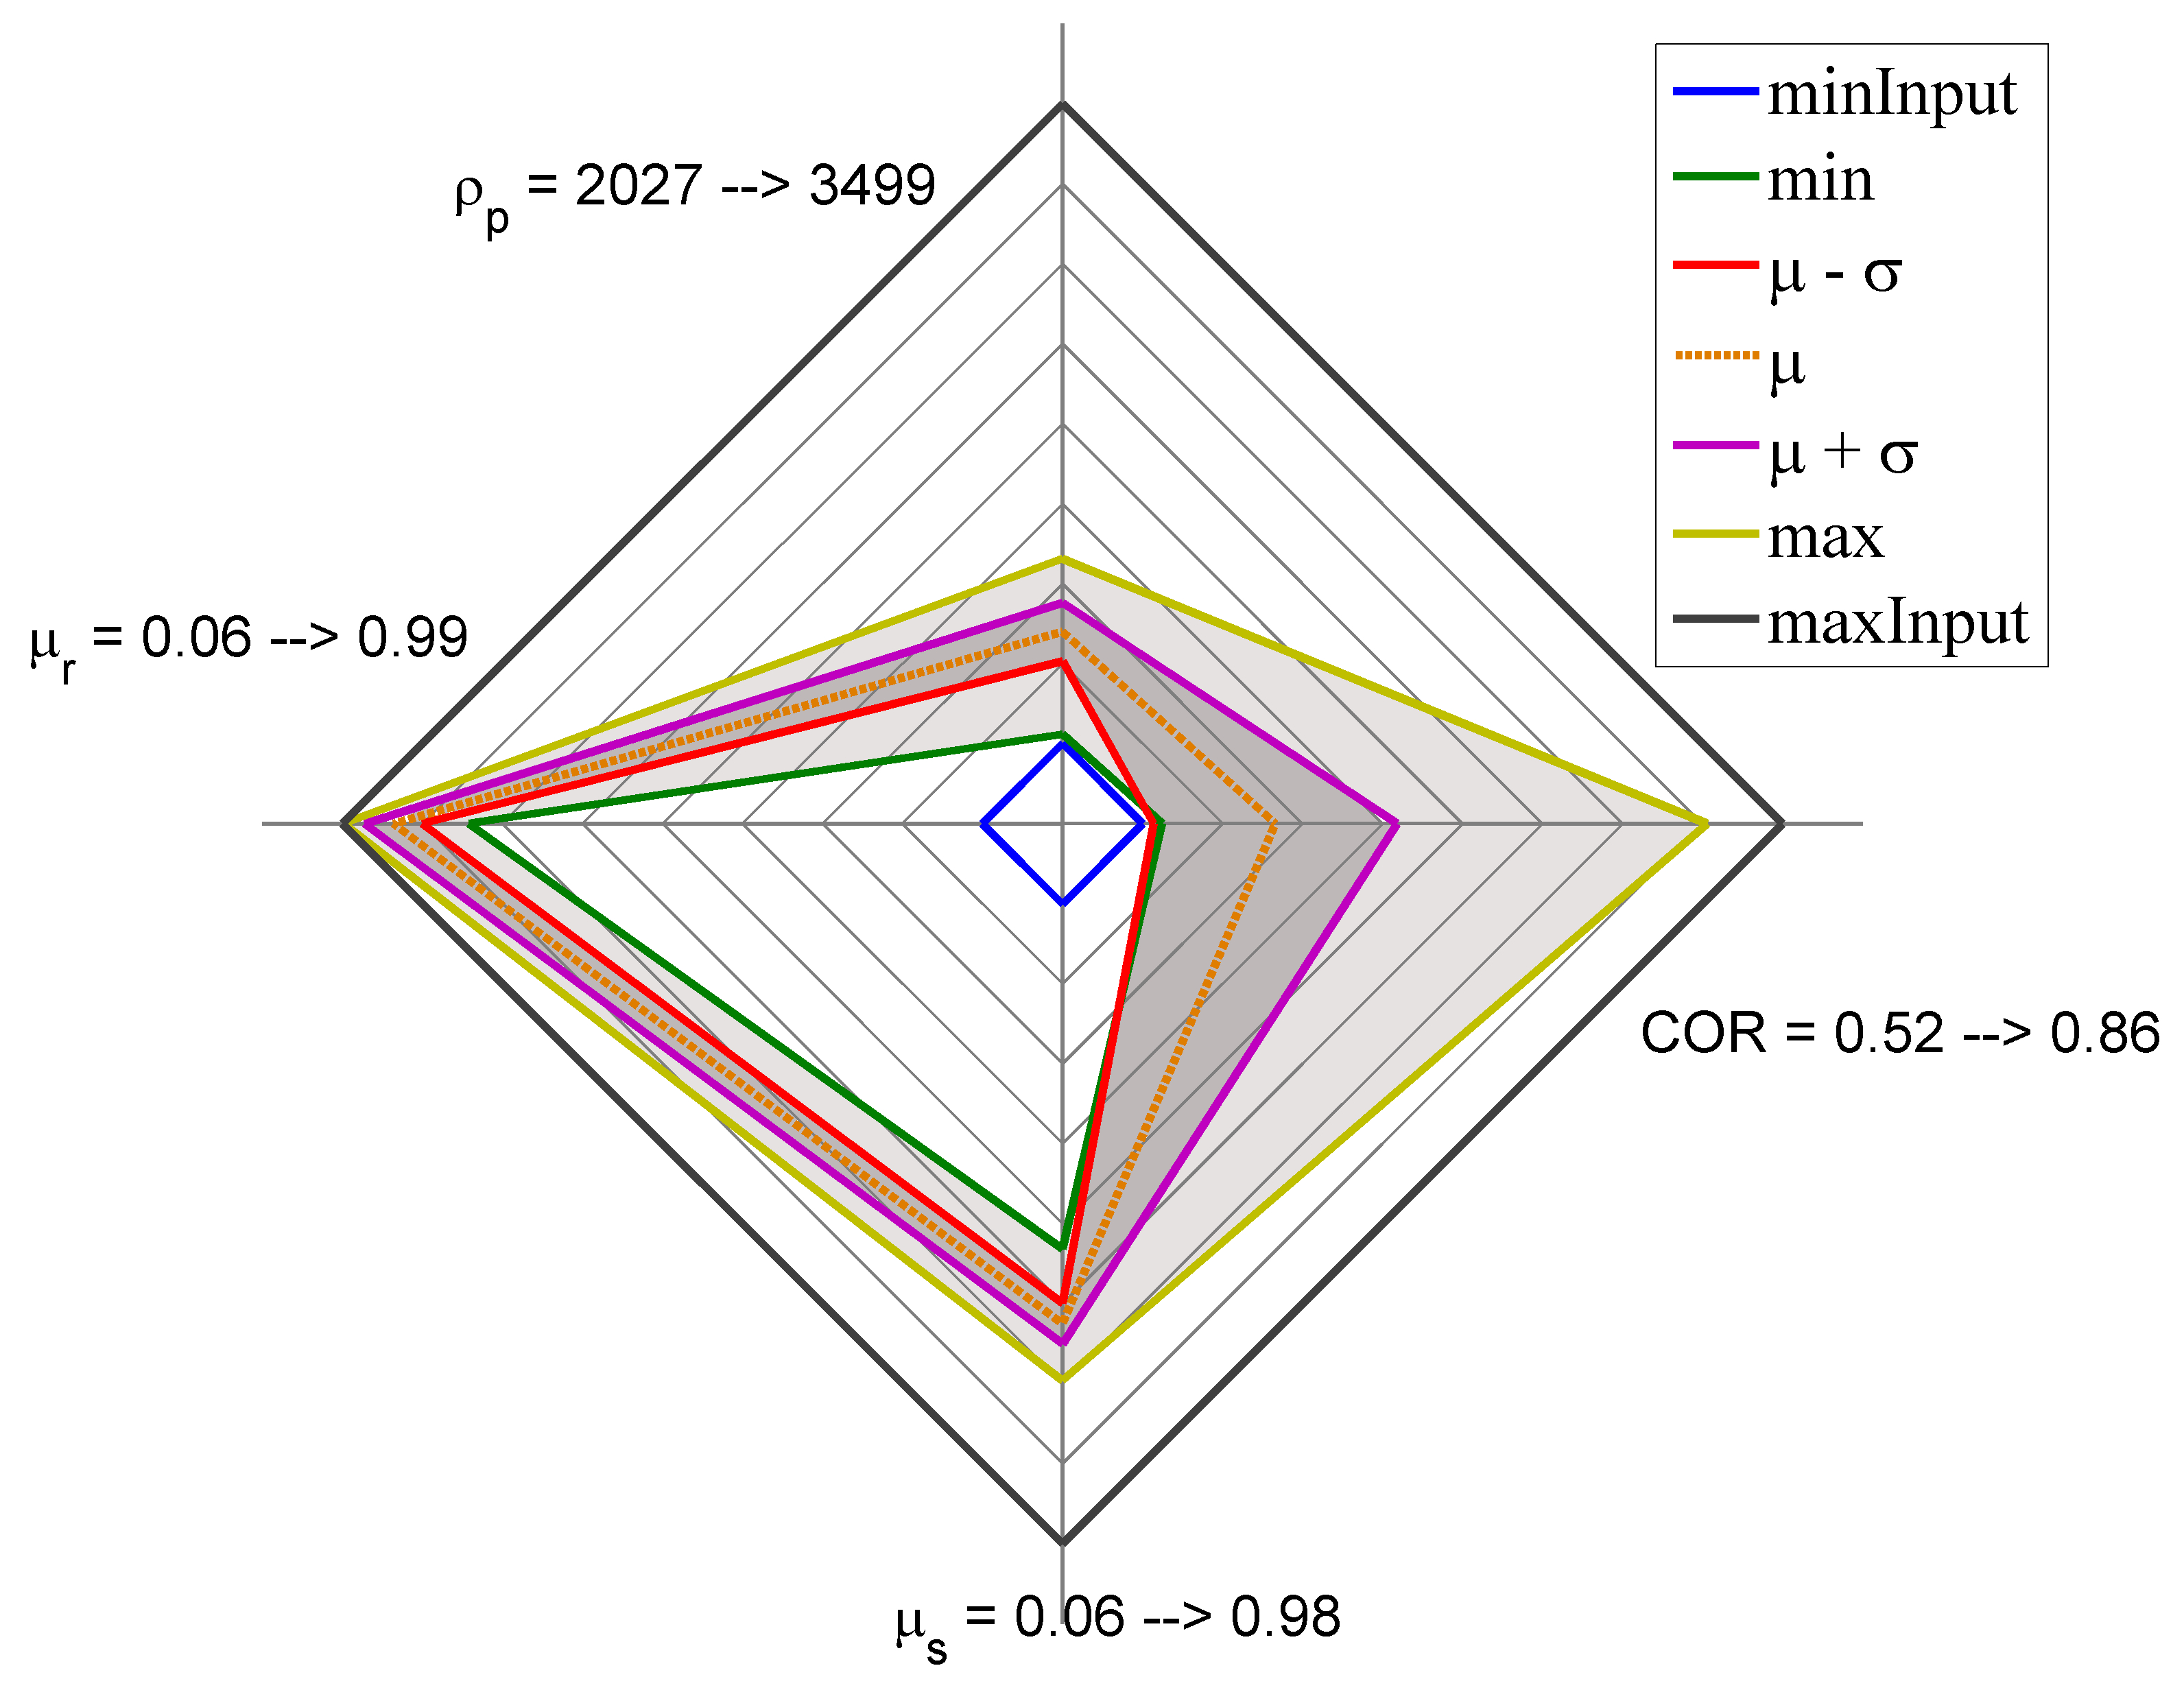
\includegraphics[width=.45\columnwidth]{images/original/33radarpirker1schulze10070aor}} \\
 \caption{Radar plots}
\label{fig:41schulze10070aor}
\end{figure}
